%% main.tex — Πρότυπο Εργασίας Πανεπιστημίου Πειραιώς
%% Μεταγλώττιση με: pdflatex main.tex (εκτέλεση δύο φορές για περιεχόμενα/αναφορές)
%%
\documentclass{unipi-assignment}

% ─── Πρόσθετα πακέτα ─────────────────────────────────────────────────────
\usepackage{lipsum}        % Dummy κείμενο (αφαιρέστε στο τελικό έγγραφο)
\usepackage{csquotes}      % Εισαγωγικά

% ─── Μεταδεδομένα εγγράφου ───────────────────────────────────────────────
\doctitle{Επιστημονική Συγγραφή στην Εκπαίδευση}       % Κεφαλίδα αριστερά
\docauthor{Ονοματεπώνυμο Φοιτητή}                     % Κεφαλίδα δεξιά

% Πεδία σελίδας τίτλου
\university{ΠΑΝΕΠΙΣΤΗΜΙΟ ΠΕΙΡΑΙΩΣ}
\school{ΣΧΟΛΗ ΤΕΧΝΟΛΟΓΙΩΝ ΠΛΗΡΟΦΟΡΙΚΗΣ ΚΑΙ ΕΠΙΚΟΙΝΩΝΙΩΝ}
\department{ΤΜΗΜΑ ΠΛΗΡΟΦΟΡΙΚΗΣ}
\coursetitle{Εργασία Μαθήματος}
\coursename{Επιστημονική Συγγραφή στην Εκπαίδευση}
\essaytitle{}
\studentname{}
\fathername{}
\studentid{Π/ΧΧΧΧΧ}
\submissiondate{Μήνας Έτος}

% ═════════════════════════════════════════════════════════════════════════
\begin{document}

% ─── Σελίδα Τίτλου (χωρίς κεφαλίδα/υποσέλιδο, χωρίς αρίθμηση) ────────────
\maketitlepage

% ─── Προκαταρκτικές Σελίδες (λατινική αρίθμηση από το copyright) ─────────
\frontmatter

% ─── Σελίδα Copyright (κεφαλίδα + υποσέλιδο, λατινική αρίθμηση) ───────────
\makecopyrightpage

% --- Περίληψη ---
% --- Περίληψη ---
\sectionunnumbered{Περίληψη}

\begin{indented}
  % Γράψτε την περίληψή σας εδώ. Η περίληψη πρέπει να συνοψίζει τους κύριους
  % στόχους, τις μεθόδους, τα αποτελέσματα και τα συμπεράσματα της εργασίας
  % με περιεκτικό τρόπο. Συνήθως κυμαίνεται από 150 έως 300 λέξεις.
\end{indented}

\vspace{160pt}
{\itshape\color{heading1color}Λέξεις Κλειδιά:\/}
\clearpage
\hbox{}%
\clearpage


% --- Πίνακας Περιεχομένων ---
\tableofcontents

\clearpage

% --- Κατάλογος Εικόνων ---
\listoffigures

\clearpage

% --- Κατάλογος Πινάκων ---
\listoftables

\clearpage

% --- Κατάλογος Διαγραμμάτων ---
\listofdiagrams

\clearpage

% ─── Κύριο Μέρος (αραβική αρίθμηση, ξεκινώντας από το 1) ─────────────────
\mainmatter

% --- Εισαγωγή ---
% --- Εισαγωγή ---
\sectionunnumbered{Εισαγωγή}

Προτεινόμενος τρόπος παρουσίασης της βιβλιογραφίας για:

\begin{indented}
  \begin{itemize}
    \item Περιοδικά: Δείτε την αναφορά~\cite{wu2004}
    \item Βιβλία και μονογραφίες: Δείτε την αναφορά~\cite{levenspiel2002}   
    \item Πρακτικά Συνεδρίων: Δείτε την αναφορά~\cite{bock1984}
    \item Κείμενο συγγράμματος με πολλούς συγγραφείς: Δείτε την αναφορά~\cite{deuflhard1987}  
  \end{itemize}  
\end{indented}


% ═══════════════════════════════════════════════════════════════════════
% ΚΕΦΑΛΑΙΟ 1
% ═══════════════════════════════════════════════════════════════════════
% ═══════════════════════════════════════════════════════════════════════
% ΚΕΦΑΛΑΙΟ 1
% ═══════════════════════════════════════════════════════════════════════
\section{Τίτλος Κεφαλαίου}

\bigskip

\subsection{Τίτλος Υποκεφαλαίου}

\bigskip

\subsubsection{Τίτλος \ldots}

\bigskip

% Παράδειγμα: εικόνα εντός κειμένου
\begin{figure}[htbp]
  \centering
  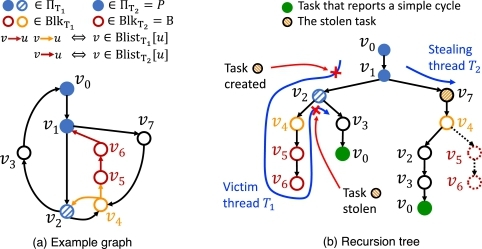
\includegraphics[width=0.7\textwidth]{images/figure-1.1.jpg}
  \caption{Περιγραφή πρώτης εικόνας πρώτου κεφαλαίου.}
  \label{fig:1.1}
\end{figure}

\subsubsection{Τίτλος \ldots}

\bigskip

\subsubsection{Τίτλος \ldots}

\bigskip

% Παράδειγμα: εικόνα εντός κειμένου
\begin{figure}[htbp]
  \centering
  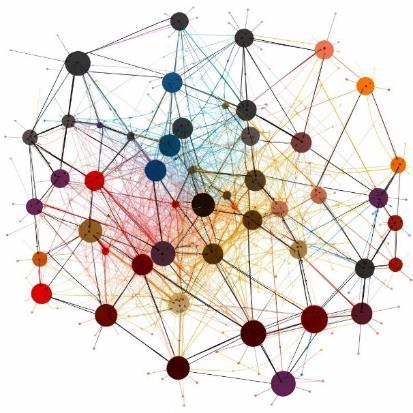
\includegraphics[width=0.5\textwidth]{images/figure-1.2.jpg}
  \caption{Περιγραφή δεύτερης εικόνας πρώτου κεφαλαίου.}
  \label{fig:1.2}
\end{figure}

\subsection{Τίτλος Υποκεφαλαίου}

\bigskip

\begin{indented}
  % Κείμενο σώματος με εσοχή
\end{indented}

\subsubsection{Τίτλος \ldots}

\bigskip

\subsubsection{Τίτλος \ldots}

\bigskip

\subsubsection{Τίτλος \ldots}

\bigskip

\subsection{Τίτλος Υποκεφαλαίου}

\bigskip

\subsubsection{Τίτλος \ldots}

\bigskip

\subsubsection{Τίτλος \ldots}

\bigskip

\subsubsection{Τίτλος \ldots}

\bigskip



% ═══════════════════════════════════════════════════════════════════════
% ΚΕΦΑΛΑΙΟ 2
% ═══════════════════════════════════════════════════════════════════════
% ═══════════════════════════════════════════════════════════════════════
% ΚΕΦΑΛΑΙΟ 2
% ═══════════════════════════════════════════════════════════════════════
\section{Τίτλος Κεφαλαίου}

\bigskip

\subsection{Τίτλος Υποκεφαλαίου}

\bigskip

\subsubsection{Τίτλος \ldots}

\bigskip

\subsubsection{Τίτλος \ldots}

\bigskip

% Παράδειγμα: εικόνα εντός κειμένου
\begin{figure}[htbp]
  \centering
  
\includegraphics[width=0.7\textwidth]{images/figure-2.1.jpg}
  \caption{Περιγραφή πρώτης εικόνας δεύτερου κεφαλαίου.}
  \label{fig:2.1}
\end{figure}

\subsubsection{Τίτλος \ldots}

\bigskip

\subsection{Τίτλος Υποκεφαλαίου}

\bigskip

\subsubsection{Τίτλος \ldots}

\bigskip

\subsubsection{Τίτλος \ldots}

\bigskip

\subsubsection{Τίτλος \ldots}

\bigskip

\subsection{Τίτλος Υποκεφαλαίου}

\bigskip

\subsubsection{Τίτλος \ldots}

\bigskip

\subsubsection{Τίτλος \ldots}

\bigskip

\subsubsection{Τίτλος \ldots}

\bigskip



% ═══════════════════════════════════════════════════════════════════════
% ΚΕΦΑΛΑΙΟ 3
% ═══════════════════════════════════════════════════════════════════════
% ═══════════════════════════════════════════════════════════════════════
% ΚΕΦΑΛΑΙΟ 3
% ═══════════════════════════════════════════════════════════════════════
\section{Τίτλος Κεφαλαίου}

\bigskip

\subsection{Τίτλος Υποκεφαλαίου}

\bigskip

\subsubsection{Τίτλος \ldots}

\bigskip

\subsubsection{Τίτλος \ldots}

\bigskip

\subsubsection{Τίτλος \ldots}

\bigskip

\subsection{Τίτλος Υποκεφαλαίου}

\bigskip

\subsubsection{Τίτλος \ldots}

\bigskip

\subsubsection{Τίτλος \ldots}

\bigskip

\subsubsection{Τίτλος \ldots}

\bigskip

% Παράδειγμα: εικόνα
\begin{figure}[htbp]
  \centering
  
\includegraphics[width=0.7\textwidth]{images/figure-3.1.jpg}
  \caption{Περιγραφή πρώτης εικόνας τρίτου κεφαλαίου.}
  \label{fig:3.1}
\end{figure}

\subsection{Τίτλος Υποκεφαλαίου}

\bigskip

\subsubsection{Τίτλος \ldots}

\bigskip

\subsubsection{Τίτλος \ldots}

\bigskip

\subsubsection{Τίτλος \ldots}

\bigskip



% ═══════════════════════════════════════════════════════════════════════
% ΚΕΦΑΛΑΙΟ 4
% ═══════════════════════════════════════════════════════════════════════
% ═══════════════════════════════════════════════════════════════════════
% ΚΕΦΑΛΑΙΟ 4
% ═══════════════════════════════════════════════════════════════════════
\section{Τίτλος Κεφαλαίου}

\bigskip

\subsection{Τίτλος Υποκεφαλαίου}

\bigskip

\subsubsection{Τίτλος \ldots}

\bigskip

\subsubsection{Τίτλος \ldots}

\bigskip

\subsubsection{Τίτλος \ldots}

\bigskip

\subsection{Τίτλος Υποκεφαλαίου}

\bigskip

\subsubsection{Τίτλος \ldots}

\bigskip

% Παράδειγμα: διάγραμμα (προσαρμοσμένο float)
\begin{diagram}[htbp]
  \centering
  
\includegraphics[width=0.7\textwidth]{images/diagram-4.1.jpg}
  \caption{Πρώτο διάγραμμα}
  \label{diag:4.1}
\end{diagram}

\subsubsection{Τίτλος \ldots}

\bigskip

% Παράδειγμα: πίνακας δεδομένων
\begin{table}[htbp]
  \centering
  \caption{Πρώτος πίνακας}
  \label{tab:4.1}
  \begin{tabular}{lccc}
    \toprule
    \textbf{Είδος} & \textbf{Τιμή 1} & \textbf{Τιμή 2} & \textbf{Τιμή 3} \\
    \midrule
    Α & 0.93 & 1.28 & 2.47 \\
    Β & 0.82 & 1.39 & 2.89 \\
    Γ & 0.75 & 1.32 & 3.14 \\
    \bottomrule
  \end{tabular}
\end{table}

\subsubsection{Τίτλος \ldots}

\bigskip

\begin{indented}
  % Κείμενο σώματος με εσοχή
\end{indented}

\subsection{Τίτλος Υποκεφαλαίου}

\bigskip

\subsubsection{Τίτλος \ldots}

\bigskip

\subsubsection{Τίτλος \ldots}

\bigskip

% Παράδειγμα: δεύτερο διάγραμμα
\begin{diagram}[H]
  \centering
  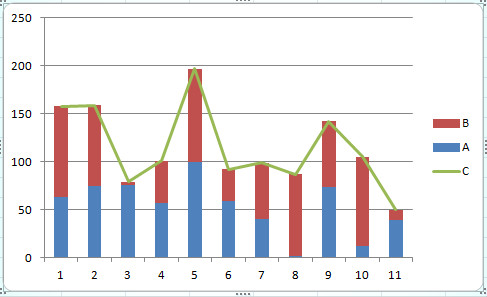
\includegraphics[width=0.7\textwidth]{images/diagram-4.2.jpg}
  \caption{Δεύτερο διάγραμμα}
  \label{diag:4.2}
\end{diagram}

\subsubsection{Τίτλος \ldots}

\bigskip

% Παράδειγμα: δεύτερος πίνακας δεδομένων
\begin{table}[H]
  \centering
  \caption{Δεύτερος πίνακας}
  \label{tab:4.2}
  \begin{tabular}{lccc}
    \toprule
    \textbf{Είδος} & \textbf{Τιμή 1} & \textbf{Τιμή 2} & \textbf{Τιμή 3} \\
    \midrule
    Α & 0.93 & 1.28 & 2.47 \\
    Β & 0.82 & 1.39 & 2.89 \\
    Γ & 0.75 & 1.32 & 3.14 \\
    \bottomrule
  \end{tabular}
\end{table}



% ═══════════════════════════════════════════════════════════════════════
% ΣΥΜΠΕΡΑΣΜΑΤΑ (χωρίς αρίθμηση)
% ═══════════════════════════════════════════════════════════════════════
% ═══════════════════════════════════════════════════════════════════════
% ΣΥΜΠΕΡΑΣΜΑΤΑ (χωρίς αρίθμηση)
% ═══════════════════════════════════════════════════════════════════════
\sectionunnumbered{Συμπεράσματα}

% Γράψτε τα συμπεράσματά σας εδώ.


% ═══════════════════════════════════════════════════════════════════════
% ΒΙΒΛΙΟΓΡΑΦΙΑ (χωρίς αρίθμηση)
% ═══════════════════════════════════════════════════════════════════════
\bibliographystyle{unsrt}
\bibliography{references}

% ═══════════════════════════════════════════════════════════════════════
% ΠΑΡΑΡΤΗΜΑΤΑ (επικεφαλίδα χωρίς αρίθμηση, έπειτα παραρτήματα με γράμματα)
% ═══════════════════════════════════════════════════════════════════════
% ═══════════════════════════════════════════════════════════════════════
% ΠΑΡΑΡΤΗΜΑΤΑ (επικεφαλίδα χωρίς αρίθμηση, έπειτα παραρτήματα με γράμματα)
% ═══════════════════════════════════════════════════════════════════════
\sectionunnumbered{Παραρτήματα}

\newpage

\makeappendixheading{}

% Περιεχόμενο Παραρτήματος Α


\newpage

\makeappendixheading{}

% Περιεχόμενο Παραρτήματος Β


\newpage


\end{document}
